% !TeX spellcheck = en_GB
%!TEX root = ../thesis.tex

\chapter{Introduction} \label{ch:intro} 

\begin{chapterabstract}
	
	In this Chapter, we give a brief introduction to the topics addressed in this thesis. We first outline the principle of forming defect modes by engineering periodic patterns in various media. We then show how this may be extended by drawing on concepts from the field of topological insulators to arrive at modes with otherwise inaccessible properties. 
	%
	Many of the modes' potential applications include some kind of time-dependent driving. This may be a modulation of the system parameters, a signal to be sensed, or a combination of both. We shall see that the modes then obey nonlinear ordinary differential equations of motion. While these are in general very hard to solve, it is possible to construct an effective approach by focusing on systems which behave harmonically in time.
	%
	While the methods used in the spatial and temporal domains are rather different, their results are complementary by nature. The potential uses of novel topological modes benefit from understanding their behaviour beyond the linear limit and vice versa.

	%
	\tcblower
	%
	Parts of this Chapter are adapted from Refs.~\cite{Kosata_2022a, Kosata_2021}.
\end{chapterabstract}

\section{Mode engineering in patterned media} \label{sec:intro_spatial}

Much of the work presented in this thesis was spurred by the recent immense advancements in creating localised, low-dissipation modes in classical media. Let us first introduce the concept of defect modes. Originally realised in photonic crystals~\cite{Joannopoulos_1997}, it relies on the existence of a bandgap in a periodic medium, which can be created by a suitable spatial pattern of features such as holes or other alterations of the material properties. If a small defect is present in the pattern, it can host one or more highly localised modes which coincide with the bulk band gap, making them effectively isolated from the surrounding medium. Due to the localisation, low losses and variability of their frequency, these modes were marked early on as candidates for laser, LEDs and other optical devices. A recent spur to the field has come from using prestressed elastic membranes as the underlying medium, resulting in defect modes with unprecedentedly high quality factors~\cite{Tsaturyan_2017}. Such modes are of tremendous technological interest to both fundamental experiments~\cite{Mason_2019, Rossi_2018} and upcoming sensing techniques~\cite{Haelg_2022, Haelg_2021, Kosata_2020}. They also provide a suiable platform for studying nonlinear behaviour~\cite{Catalini_2021}, which we turn to in Sec.~\ref{sec:intro_nonlin}. 

\subsubsection{Topology in metamaterials}

Despite their successes, the prevalent understanding of the aforementioned defect modes is quite phenomenological. Determining the modes' existence and properties usually relies on extensive numerical simulations. A viable alternative is offered by the concept of \textit{topological insulators} (TIs), where defect modes are guaranteed to appear, provided certain requirements are met. TIs are materials featuring a bandgap, which may be opened in multiple topologically distinct ways. Here we shall be interested in a subsection of this vast field -- \textit{topological boundary modes}, which occur at boundaries between topologically distinct insulator bulks. The canonical example is the quantum Hall effect, where, in the presence of a magnetic field, one-way (\textit{chiral}) modes arise at the boundary between a topological insulator and vacuum. In Fig.~\ref{fig:intro_topo}(a), despite the insulating bulk, the boundary displays unidirectional conductivity due to a single mode that crosses the bandgap. Strictly speaking, the existence of this mode follows from a topological invariant changing across the boundary~\cite{Bernevig_2013}, here the \textit{Chern number} $C$. In Fig.~\ref{fig:intro_topo}, the Chern numbers of the bands below and above the gap are marked.

The boundary mode itself may be modelled by the \textit{Jackiw-Rebbi Hamiltonian}~\cite{Jackiw_1976}. Not unique to topology, it has two key ingredients. (i) Two bands touching at a single point in $k$-space. (ii) A gap-opening \textit{mass term} which switches signs across the boundary, creating a \textit{band inversion} there. The resulting gap-crossing mode shows linear dispersion and exponential localisation at the boundary. In the quantum Hall effect, the mode's chirality reflects the breaking of time-reversal symmetry by the magnetic field. However, as shown by Kane and Mele in 2015~\cite{Kane_Mele_2005}, when TRS is present, a pair of counter-propagating one-way modes may form at a boundary between two distinct bulks -- the quantum spin Hall effect [Fig.~\ref{fig:intro_topo}(b)]. This can be modelled by two instances of the Jackiw-Rebbi Hamiltonian, thus requiring four bands in total.

\begin{figure} [h!]
	\centering
	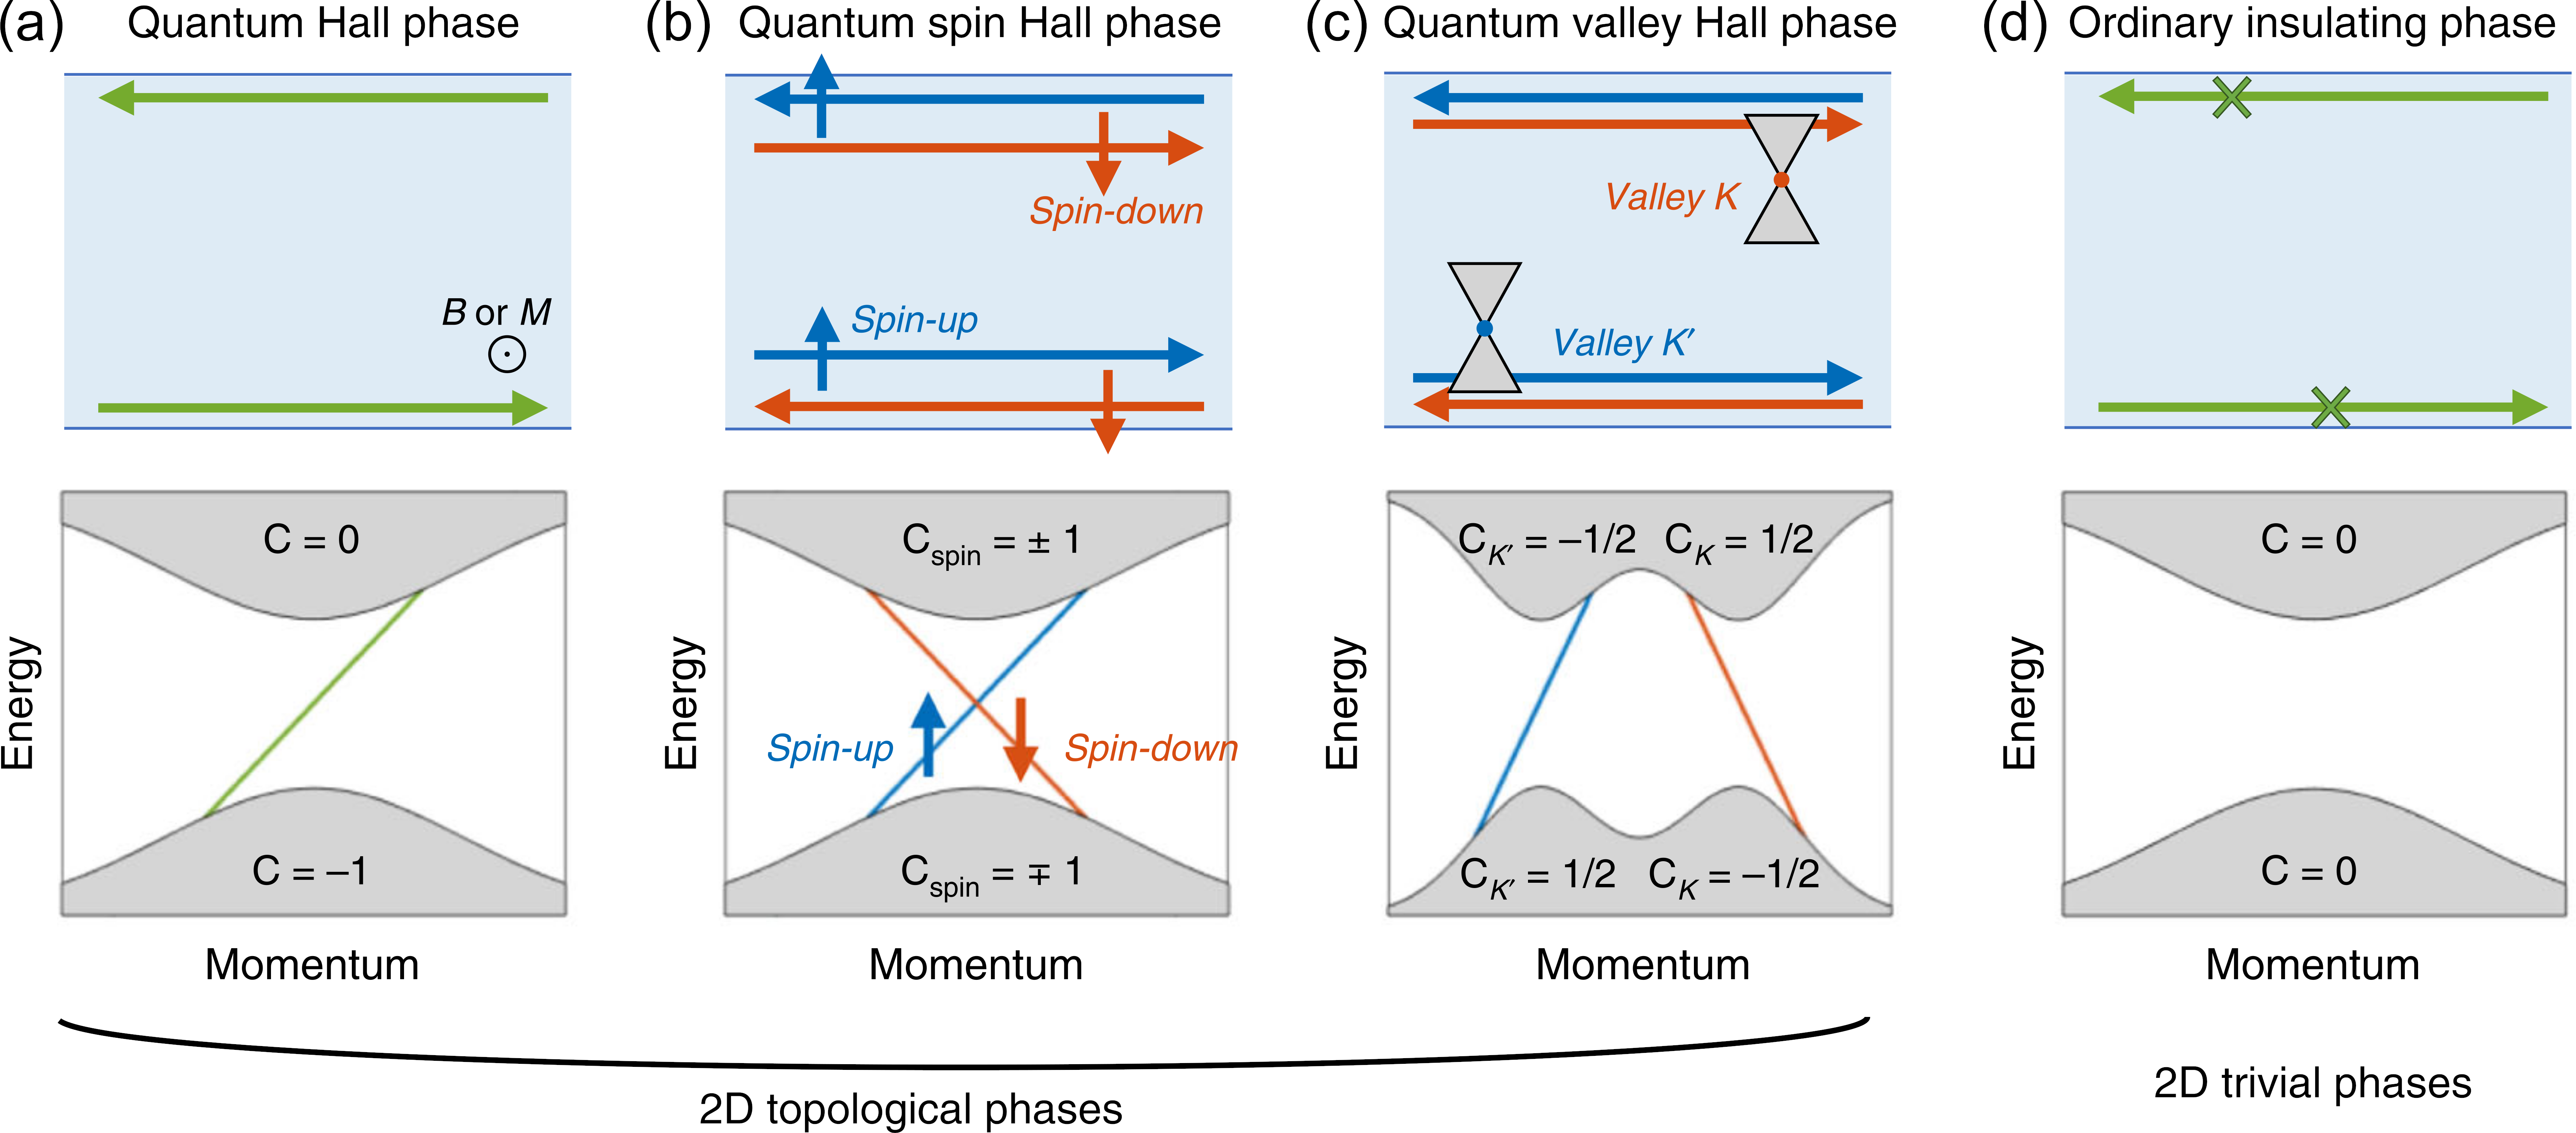
\includegraphics[width=\textwidth]{figures/intro/topological_phases_edited.png}
	\caption{The boundary modes occurring in the (a) quantum Hall, (b) quantum spin Hall, (c) quantum valley Hall effects, and (d) an ordinary insulating bulk. (a) Unidirectional boundary mode (green) in the TRS-broken system. Its dispersion has a fixed sign of the group velocity. (b) Counter-propagating boundary modes (red and blue) in the quantum spin Hall system. Their dispersion shows spin-locked group velocities, with each spin direction possessing different Chern numbers. (c) Counter-propagating boundary modes (red and blue) in the quantum valley Hall system. Their dispersion shows valley-locked group velocities, with the two valleys possessing different Chern numbers. (d) The ordinary insulating bulk does not support boundary modes. Adapted from Ref.~\cite{Kim_2020}.}
	\label{fig:intro_topo}
\end{figure}

In 2008, a classical realisation the quantum Hall effect was proposed~\cite{Haldane_2008} and demonstrated soon after~\cite{Wang_2008, Wang_2009} using a gyromagnetic material in a strong magnetic field. Subsequent realizations of topology in classical systems relied on engineering synthetic gauge fields in tight-binding (TB) models, obtained by coupling oscillator modes in space~\cite{Kraus_2012, Hafezi_2013} and/or time~\cite{Rechtsman_2013}. However, the requirement of breaking TRS turned out to be too restrictive, as the gyromagnetic effect is rather weak, and realisations beyond electromagnetism require external driving to break TRS. 

A turning point was marked by the work of Wu and Hu in 2015~\cite{Wu_Hu_2015}, which showed how to obtain pairs of counter-propagating modes by patterning a dielectric medium without breaking TRS. We recount the key ideas:%
%
\begin{enumerate}

	\item In a linear medium patterned with a suitable symmetry, band touchings (Dirac cones) are guaranteed to exist at certain points in $k$-space.

	\item Deforming the pattern to break some of its symmetries may open the Dirac cones to create a bandgap.

	\item The sign of the gapping term depends on the details of the deformation, with bulks featuring opposite gapping term signs related by band inversion. A boundary between them obeys the Jackiw-Rebbi Hamiltonian, giving rise to a pair of counter-propagating modes.

\end{enumerate}
%
The impact of this scheme can hardly be overstated. The signature topological boundary modes have been successfully demonstrated in photonic~\cite{Li_2018, Ozawa_2019}, electrical~\cite{Ningyuan_2015, Hofmann_2019}, phononic~\cite{Nash_2015,  Mousavi_2015, Huber_2016}, acoustic~\cite{He_2016, Ma_2019}, atomic~\cite{Cooper_2019} and polaritonic~\cite{Milicevic_2015} systems, bringing the field closer to potential applications. Many material patterns are used throughout the literature, including the square, Kagome, hexagonal and honeycomb lattices. Depending on the pattern and its symmetry breaking, the quantum spin Hall effect or the closely-related quantum valley Hall effect [Fig.~\ref{fig:intro_topo}(c)] can be mimicked. 

More recently, the concept of topological modes has been extended to higher-order TIs (HOTIs)~\cite{Kraus_2013,Benalcazar_2017a,Benalcazar_2017b,Petrides_2018, Zilberberg_2018, Benalcazar_2019, Calugaru_2019, Fukui_2019, Petrides_2020}. In a $d$-dimensional HOTI, topological modes of dimension $d-2$ and lower may appear. HOTIs have been experimentally demonstrated by emulating tight-binding models in a variety of platforms~\cite{Imhof_2018, Noh_2018, Schindler_2018, Serra-Garcia_2018, Fan_2019, Xue_2019, Xie_2018, Zhang_2019, Zhang_2020, Zhou_2020}. In this thesis, we describe a group-theoretical framework that identifies suitable material patterns and their symmetry breaking to design instances of both TIs and HOTIs. 

Finally, a note of caution is in order. Although their development has been extremely influential, the topological nature of the aforementioned modes is a matter of ongoing debate~\cite{Saba_2020, Qian_2018}. This thesis does not deal with these issues, focusing merely on the boundary mode models and their symmetries. 

\section{Nonlinear dynamical systems} \label{sec:intro_nonlin}

The temporal behaviour of a system consisting of one or more modes is described by a set of ordinary differential equations (ODEs). While linear approximations are undoubtedly the bread and butter of physics, any realistic system is nonlinear when a wide enough range of operating conditions is considered. Nonlinear ODEs host unique phenomena, including bifurcations, internal resonance, synchronisation, and chaos~\cite{vibrations1950jj,dykman1975theory,Strogatz,Rand_2005, Nayfeh_Mook,Schuster2009,Mangussi2016}. In particular, explicitly time-dependent or \textit{non-autonomous} nonlinear ODEs describe driven-dissipative systems, which commonly exhibit harmonic time dependence of the system parameters and/or external drives~\cite{Richards}, see Fig.~\ref{fig:intro_setup}(a). 
Such systems appear in a range of active fields, such as modal analysis in structural dynamics~\cite{Ewins2000,Kerschen2006}, electric circuits~\cite{Rohde2005,Rubiola2008,Fallis2003}, nonlinear optics~\cite{Haken1975,Shen2002,del2007optical,Rodriguez2016,DelPino2016,Sounas2018,Zambon_2020,peters2021limit}, optomechanics~\cite{Aspelmeyer2014,Pelka2020,Burgwal2020,Roque2020}, micro- and nanomechanics~\cite{Poot2012,Papariello_2016,Guttinger2017,Chen2017,Houri2019,Houri2020,Yang_2021a, Yang_2021b, Mohammadi2020,Huber_2020,2018ApPhL.112w3105E,2021arXiv210911943H, Kosata_2020}, oscillator networks~\cite{2016PhRvA..93d3827O,2019PhRvL.123l4301H,Ozawa2019,del2021non,2022arXiv220106315P, Kosata_2021},  Ising machines~\cite{Wang2013,Bello2019a,CalvaneseStrinati2019,2019PhRvL.123y4102F,CalvaneseStrinati2020,Heugel_2022}, and many-body light-matter systems~\cite{griffin1996bose,Carusotto2013,Soriente2018,Kirton2019,Soriente2020,Soriente2021,2021PhRvX..11d1046F}.

\begin{figure} [ht!]
	\centering
	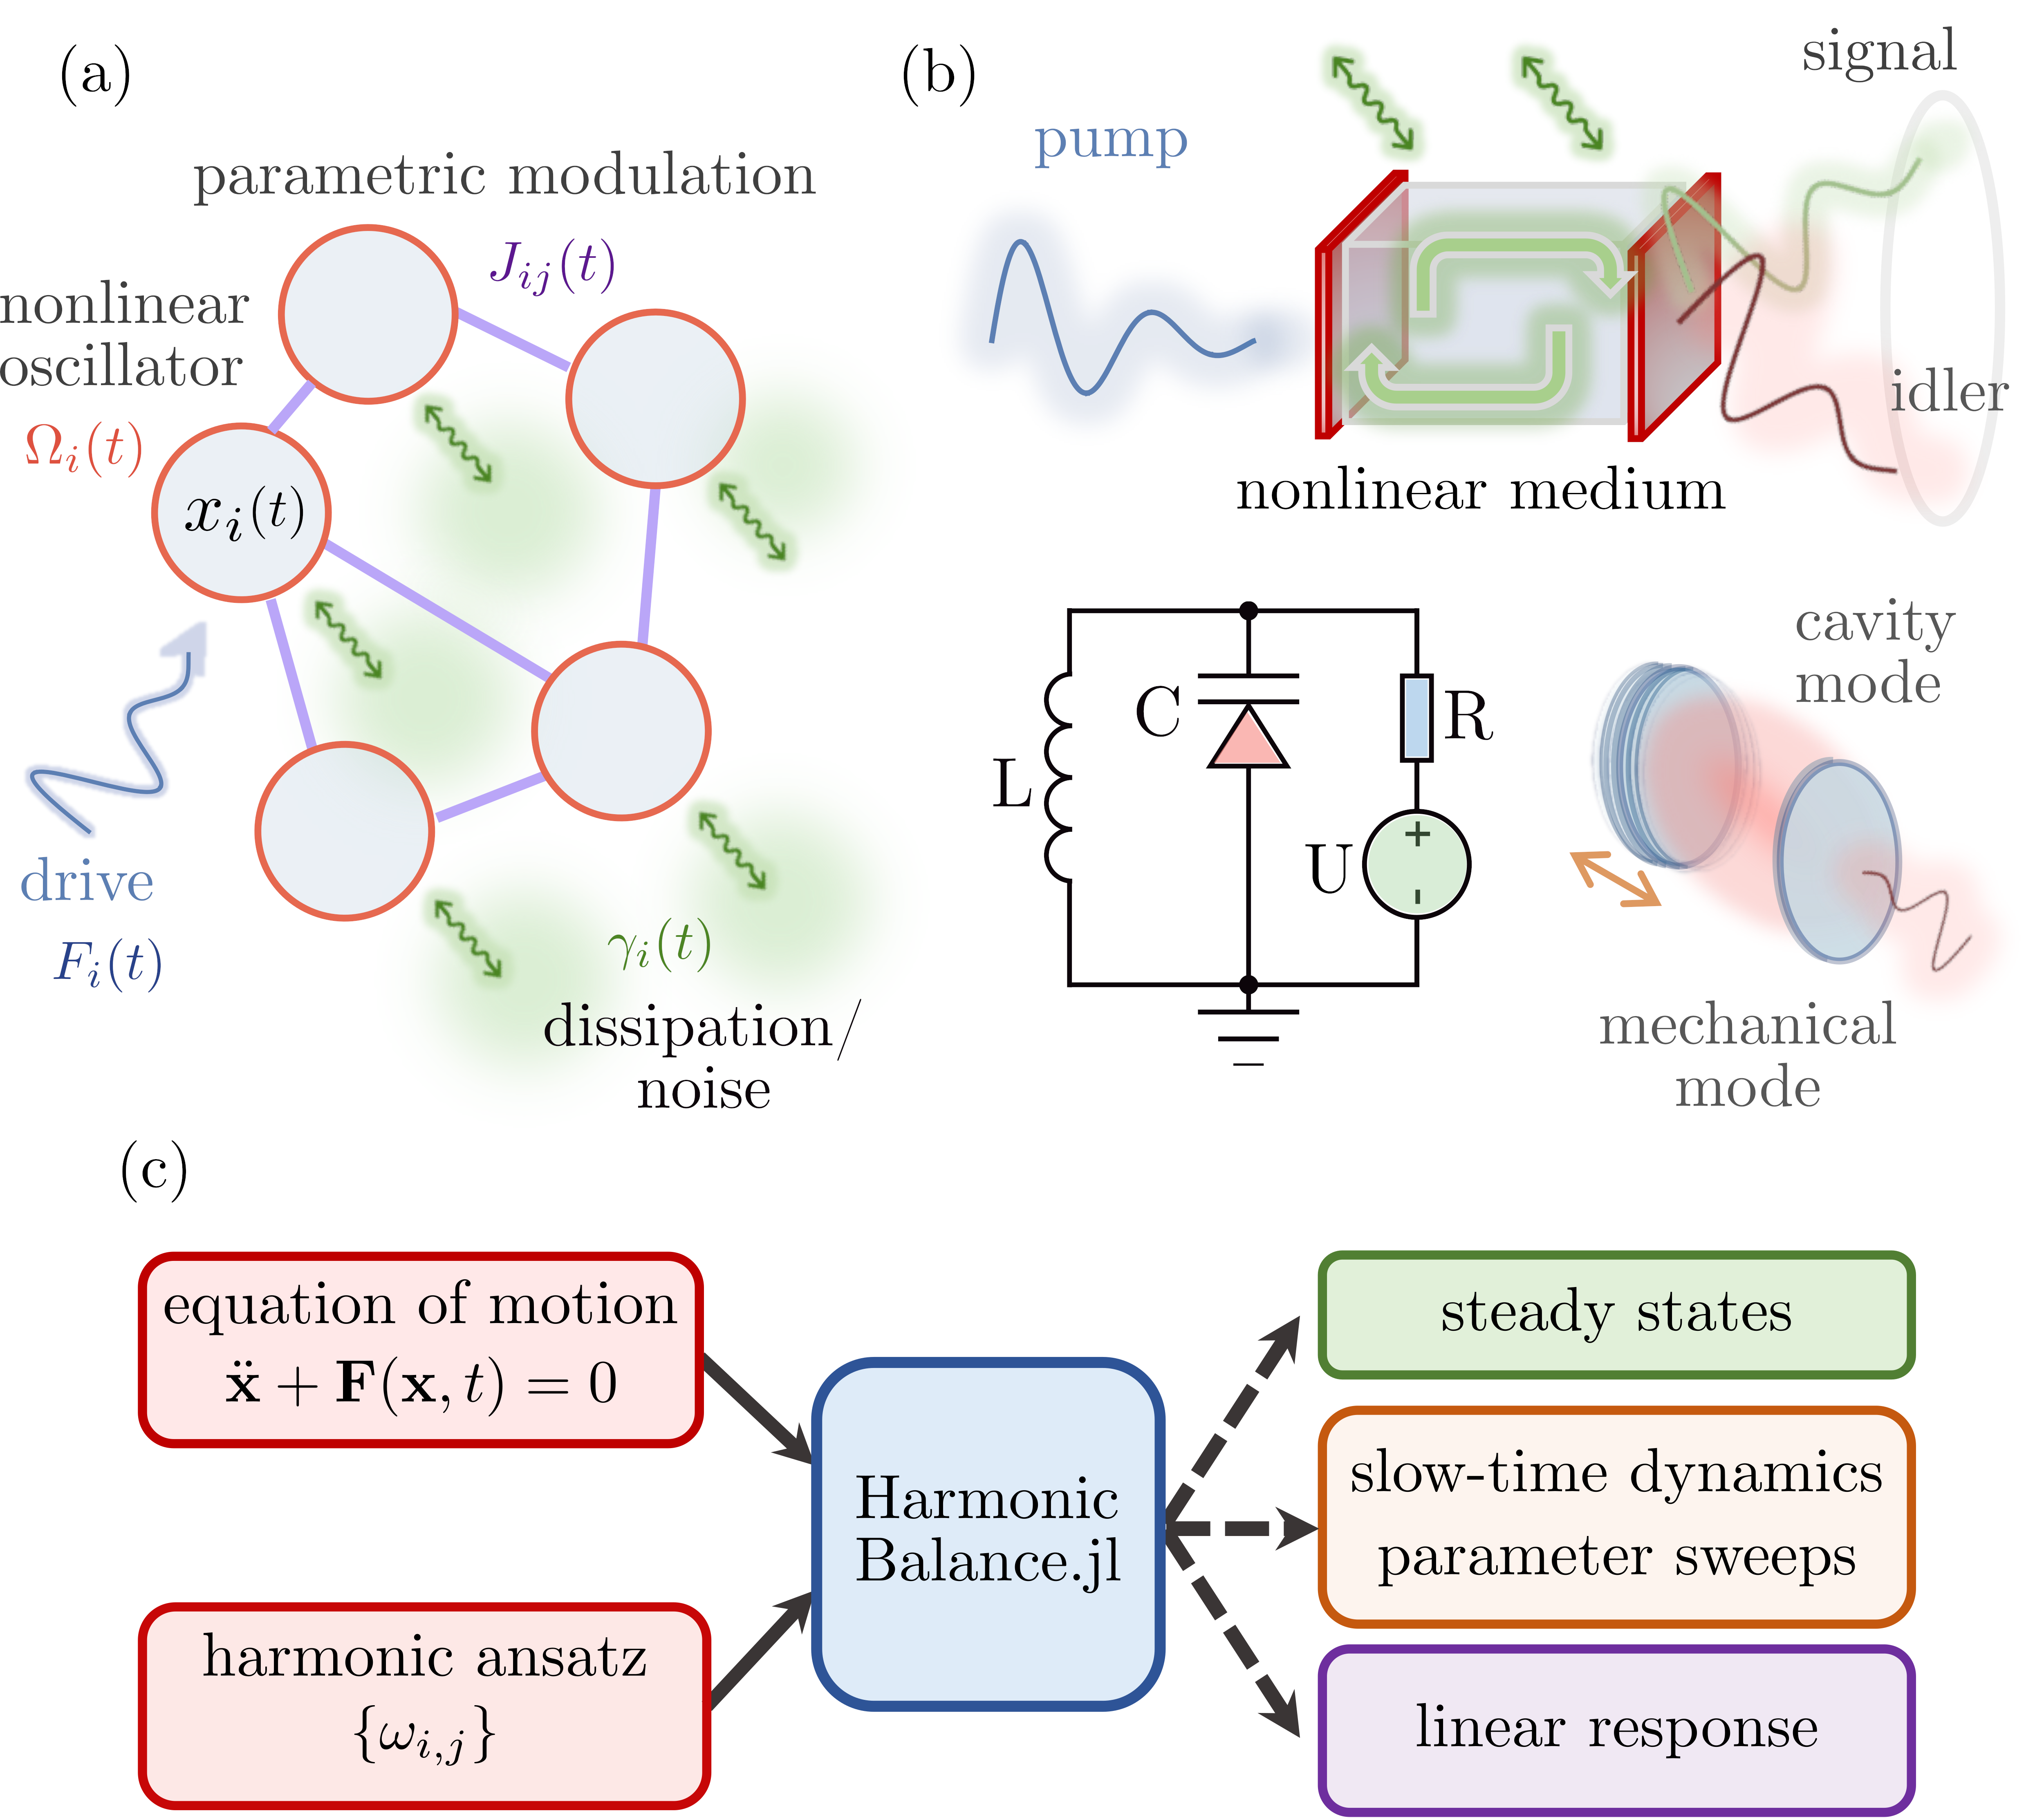
\includegraphics[width=\textwidth]{figures/intro/flow_diag.png}
	\caption{(a) A generic driven dissipative system: coupled nonlinear oscillators (circles) with amplitudes $x_i(t)$, time-varying natural frequencies $\Omega_i(t)$, and coupling amplitudes $J_{ij}(t)$. System-environment interactions, parameterised by $\gamma_i(t)$, lead to fluctuations and dissipation. Harmonic drives with amplitudes $F_i(t)$ excite and modify the system's response. (b) Examples of nonlinear devices: (top) light fields interacting with nonlinear media, (bottom, left) driven nonlinear electric RLC circuits, and (bottom right) optomechanical oscillators. (c) Core functionality of HarmonicBalance.jl. Adapted from Ref.~\cite{Kosata_2022b}.}
	\label{fig:intro_setup}
\end{figure} 

Provided dissipation is present, a harmonically-driven system will, given sufficient time, settle to a \textit{steady state}. This is typically an oscillatory response that does not change further in time. Arguably the simplest way of finding the steady states is to use a numerical ODE solver, which propagates the system in time, essentially simulating an experiment. However, in nonlinear problems, a system may display a multitude of steady states -- \textit{multistability}. The observed response then depends purely on the initial conditions. To obtain the complete steady state diagram, one must resort to some manner of sampling the space of initial conditions. Besides being time-consuming, this approach offers no guarantee of finding the complete set of steady states.

A different strategy is to transform the system into Fourier space\footnote{This may also be viewed a generalisation of the \textit{rotating frame} concept.}, where an oscillatory response appears constant. Truncating the Fourier space to a few components of interest, finding the steady states then necessitates solving a set of coupled algebraic equations. This is still a formidable task~\cite{Bernshtein1975,sturmfels2002solving,cox2005solving}, as iterative root-finding methods give roots one by one, again with no guarantee of finding all of them. As a result, full characterisation of all but the simplest systems presents a challenge.  Fortunately, the equations often turn out to be coupled polynomials, which may be solved completely using the method of homotopy continuation~\cite{Sommese2005,Breiding_2018,timme2021numerical} -- this is the direction explored in this thesis. 

The ability to compute steady state diagrams is an ideal starting point for analysing a nonlinear harmonically-driven system and its applications. Experimentally observable phenomena such as hysteresis and noise-induced switching dynamics~\cite{Leuch_2016, Heugel_2019, Margiani2021} are all captured by relevant cuts through the solution manifold. Depending on the dimensionality of the truncated Fourier space, phenomena such as frequency conversion and period doubling may be described. Applications such as sensing go one step further by introducing a perturbation of the steady states and investigating the resulting response. Contemporary research topics such as the emergence of aperiodic solutions and frequency combs may also be addressed within truncated Fourier space, provided a time-dependent drift of the steady state is allowed. In this thesis, we bring these concepts under one roof to construct a self-consistent framework. We shall see that this allows us to solve hitherto intractable problems, enabling the study of a whole class of nonlinear systems.


\section{Thesis outline and contributions}
%\addcontentsline{toc}{section}{Thesis outline and contributions}

This thesis is split into two topical parts. 

\textbf{Part \ref{part:spatial}: Spatial} concerns spatial patterning of continuous media to create modes. It makes use of the publication \cite{Kosata_2021}.

\textbf{Symmetry analysis} In Chapter \ref{ch:symmetry}, we view the creation of topological modes from a purely symmetry-oriented perspective, arriving at a general mechanism for creating first-order topological modes. 

\textbf{Second-order topology in continuous media} In Chapter \ref{ch:hoti} we use the framework of Chapter \ref{ch:symmetry} to formulate a scheme for creating second-order topological modes with technologically useful properties.

\textbf{Part \ref{part:temporal}: Temporal} concerns the behaviour of multi-mode systems in time, with a focus on nonlinear phenomena resulting from driving. It makes use of the publications \cite{Kosata_2022a, Kosata_2022b, Kosata_2020}.

\textbf{Nonlinear harmonic systems} In Chapter \ref{ch:hb} shows how spatial modes give rise to coupled differential equations. Focusing on harmonically-driven systems, we introduce the methods of harmonic balance and homotopy continuation to find steady-state responses.

\textbf{Linear response} In Chapter \ref{ch:linresp} we explore the concept of solution stability and the response of a driven system to a perturbation. 

\textbf{Solutions with broken time-translation symmetry} In Chapter \ref{ch:hopf}, we relax the hitherto assumed requirement of time-translation symmetry of the solutions. We adapt the method of harmonic balance to capture spontaneous symmetry-breaking and discuss its implications. 

\textbf{Harmonic balance in quantum mechanics} In Chapter \ref{ch:rwa}, we turn from classical to quantum formalism, discussing the rotating-wave approximation and showing its equivalence to harmonic balance. We address its known insufficiency for off-resonantly driven systems and offer a non-standard operator formalism to quantise harmonically-driven oscillators. 

\textbf{Application: spin detection via parameteric frequency conversion} In Chapter \ref{ch:spins}, we use the concepts introduced throughout this thesis for an in-depth analysis of an experimental measurement scheme. 
%

\subsection*{Contributions}
%\addcontentsline{toc}{section}{Contributions}
Here I summarize the publications that resulted from this thesis, and clarify my role in their creation.

Publication~\cite{Kosata_2020} represents my initial stage at the ETH, where I worked closely with the group of Christian Degen, in particular with Alex Eichler. Written together with Oded Zilberberg and R. Chitra, it fleshes out Alex's idea of using coupled oscillators for spin sensing and serves primarily as an accessible blueprint for experimental physicists. I also made a minor contribution to publication \cite{Grob_2019} by analysing spin dynamics for NanoMRI, which does not appear in this thesis.

I then moved into topological physics where I provided spatial mode designs to the experimental group of Albert Schliesser at the University of Copenhagen. These are currently in production and are not published. In the process, the idea of formulating a symmetry-based approach to inducing second-order topology in continuous media originated. This led to publication \cite{Kosata_2021}, under the supervision of Oded.

Publication \cite{Kosata_2022b} originated in the master's project of Tobias K\"{a}stli, which I supervised together with Anina Leuch (shared first author). A part of Tobias's thesis addressed a known shortcoming of a standard textbook method -- the rotating-wave approximation. With Anina, we went on to localise the cause, adapt the formalism for use with driven dissipative systems, and write the publication.

An integral part of my doctorate were the plentiful collaborations with experimental groups. The repeated encounters with their complicated dynamical systems spurred on the coding efforts that culminated in releasing HarmonicBalance.jl~\cite{Kosata_2022a} -- an open-source Julia package integrating many years of the group's know-how. The development was done in close collaboration with Javier del Pino (shared first author). Oded and Toni Heugel provided valuable guidance stemming from their considerable experience in the field. Ongoing maintenance and additions reflecting contemporary research problems are expected.

Publications \cite{Kosata_2018a, Kosata_2018b, Nilsen_2017} originate from before my time at the ETH and do not form a part of this thesis.


